\documentclass[11pt,a4paper]{article}

% ---------- Packages ----------
\usepackage[utf8]{inputenc}
\usepackage[T1]{fontenc}
\usepackage{lmodern}
\usepackage{amsmath,amssymb}
\usepackage{enumitem}
\usepackage{geometry}
\usepackage{fancyhdr}
\usepackage[most]{tcolorbox}   % enhanced, breakable
\usepackage{hyperref}

% ---------- Geometry ----------
\geometry{margin=2.5cm}

% ---------- Header/Footer ----------
\setlength{\headheight}{14pt}  % fancyhdr warning verhindern
\pagestyle{fancy}
\fancyhf{}
\lhead{Einführung in die Elektrotechnik}
\rhead{Wintersemester 2025}
\cfoot{\thepage}

% ---------- Exercise Environment ----------
\newcounter{exercise}
\newenvironment{exercise}[1][]
  {\refstepcounter{exercise}%
   \begin{tcolorbox}[enhanced, breakable, width=\textwidth,
     colback=blue!5!white,colframe=blue!60!black,
     fonttitle=\bfseries\large,
     title=Aufgabe~\theexercise:~#1]}
  {\end{tcolorbox}}

% ---------- Solution Environment ----------
\newif\ifshowsolutions
\showsolutionstrue  % comment to hide solutions

\newenvironment{solution}
  {\ifshowsolutions
     \begin{tcolorbox}[enhanced, breakable, width=\textwidth,
       colback=green!5!white,colframe=green!50!black,
       fonttitle=\bfseries\large,
       title=Lösung]}
  {\end{tcolorbox}\fi}

% ---------- Document ----------
\begin{document}

% ----- Header Box -----
\begin{tcolorbox}[enhanced, breakable, colback=gray!10!white,
  colframe=gray!70!black, fonttitle=\bfseries\large,
  title={Aufgabenblatt \#6}: Transformator und Transienten, sharp corners, width=\textwidth]
\begin{center}
  Besprechung: 24.11.2025
\end{center}
\end{tcolorbox}
\vspace{1cm}

% ----- Exercise 1 -----
\begin{exercise}[Idealer Transformator]
Ein idealer 480-V nach 2400-V Aufwärtstransformator liefert $50\,\text{kW}$ an eine ohmsche Last. Berechne:
\begin{enumerate}[label=\alph*)]
  \item das Windungsverhältnis
  \item den Primärstrom
  \item den Sekundärstrom
\end{enumerate}
\end{exercise}

\ifshowsolutions
\begin{solution}
\begin{enumerate}[label=\alph*)]
\item Windungsverhältnis (primär zu sekundär):
\[
\alpha = \frac{V_P}{V_S} = \frac{480\,\text{V}}{2400\,\text{V}} = 0.2
\]
\item Primärstrom:
\[
I_P = \frac{P}{V_P} = \frac{50000\,\text{W}}{480\,\text{V}} \approx 104.17\,\text{A}
\]
\item Sekundärstrom:
\[
I_S = \frac{P}{V_S} = \frac{50000\,\text{W}}{2400\,\text{V}} \approx 20.83\,\text{A}
\]
Überprüfung:
\[
\frac{I_S}{I_P} \approx 0.2
\]
\end{enumerate}

\textbf{Bemerkung:}
Für Wechselstrom würde man einfach Effektivwerte betrachten.
\end{solution}
\fi

% ----- Exercise 2 -----
\begin{exercise}[Gegenseitige Induktivität]
Berechne die gegenseitige Induktivität für folgende drei gekoppelte Spulen.

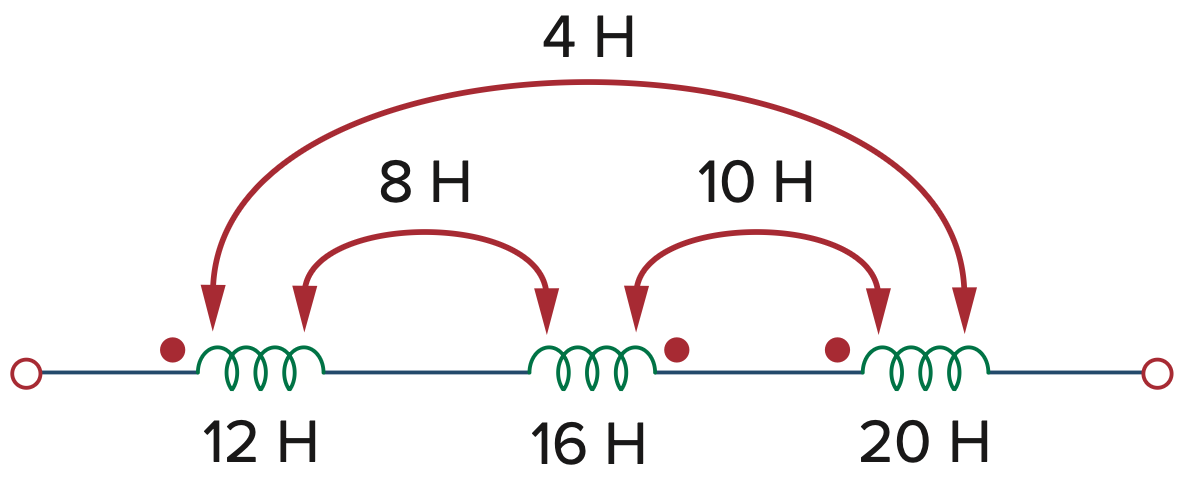
\includegraphics[width=0.7\textwidth]{figures/mutual_inductance.png}

\textbf{Hintergrund:}
Die Polarität der Gegenspannung wird durch die Ausrichtung der beiden Spulen bestimmt. Sie lässt sich mithilfe der Lenzschen Regel und der Rechte-Hand-Regel ermitteln. In Schaltplänen wird die Polarität häufig durch die Punktkonvention dargestellt: An einem Ende jeder der beiden magnetisch gekoppelten Spulen wird ein Punkt gesetzt, der die Richtung des magnetischen Flusses angibt, wenn Strom in diesen Punkt fließt. Die Konvention lautet dann: Fließt Strom in den Punkt einer Spule, so ist die Referenzpolarität der Gegenspannung in der zweiten Spule am Punkt der zweiten Spule positiv.
\end{exercise}

\ifshowsolutions
\begin{solution}
\[
\text{Gegeben: } 
\begin{cases}
L_1 = 12~\text{H},\\
L_2 = 16~\text{H},\\
L_3 = 20~\text{H},\\
M_{12} = 8~\text{H},\\
M_{23} = 10~\text{H},\\
M_{13} = 4~\text{H}.
\end{cases}
\]

Die Gesamtinduktivität eines Systems von in Reihe geschalteten, magnetisch gekoppelten Spulen hängt nicht nur von den Selbstinduktivitäten der Spulen ab, sondern auch von den Gegeninduktivitäten zwischen ihnen.

Sind zwei Spulen so verbunden, dass der von der einen erzeugte magnetische Fluss den Fluss in der anderen \emph{verstärkt}, trägt die Gegeninduktivität \emph{positiv} bei. \emph{Hemmen} sich die Flüsse, trägt die Gegeninduktivität \emph{negativ} bei.

In der gegebenen Schaltung:
\begin{enumerate}
  \item Die Punkte geben die Polarität der induzierten Spannung in jeder Spule an.
  \item Das Verbindungsmuster zeigt Folgendes:
  \begin{enumerate}
    \item \( M_{12} \) und \( M_{23} \) sind \emph{gegensätzlich} (Der Strom tritt in den gepunkteten Anschluss der einen Spule ein und verlässt ihn am gepunkteten Anschluss der anderen Spule.).
    \item \( M_{13} \) wirkt \emph{verstärkende} (Der Strom fließt in beide gepunkteten Anschlüsse.).
  \end{enumerate}
\end{enumerate}

Bei drei in Reihe geschalteten, gekoppelten Spulen ergibt sich die äquivalente Induktivität wie folgt:
\[
L_{\text{eq}} = L_1 + L_2 + L_3 + 2(\pm M_{12} \pm M_{23} \pm M_{13}),
\]
wobei die Vorzeichen davon abhängen, ob die gegenseitige Wechselwirkung unterstützend oder entgegenwirkend ist.

Aus den Polaritätsinformationen im Diagramm ergibt sich:
\[
L_{\text{eq}} = L_1 + L_2 + L_3 + 2(M_{13} - M_{12} - M_{23}) = (12 + 16 + 20 + 2(4 - 8 - 10))~\text{H} = 20~\text{H}
\]

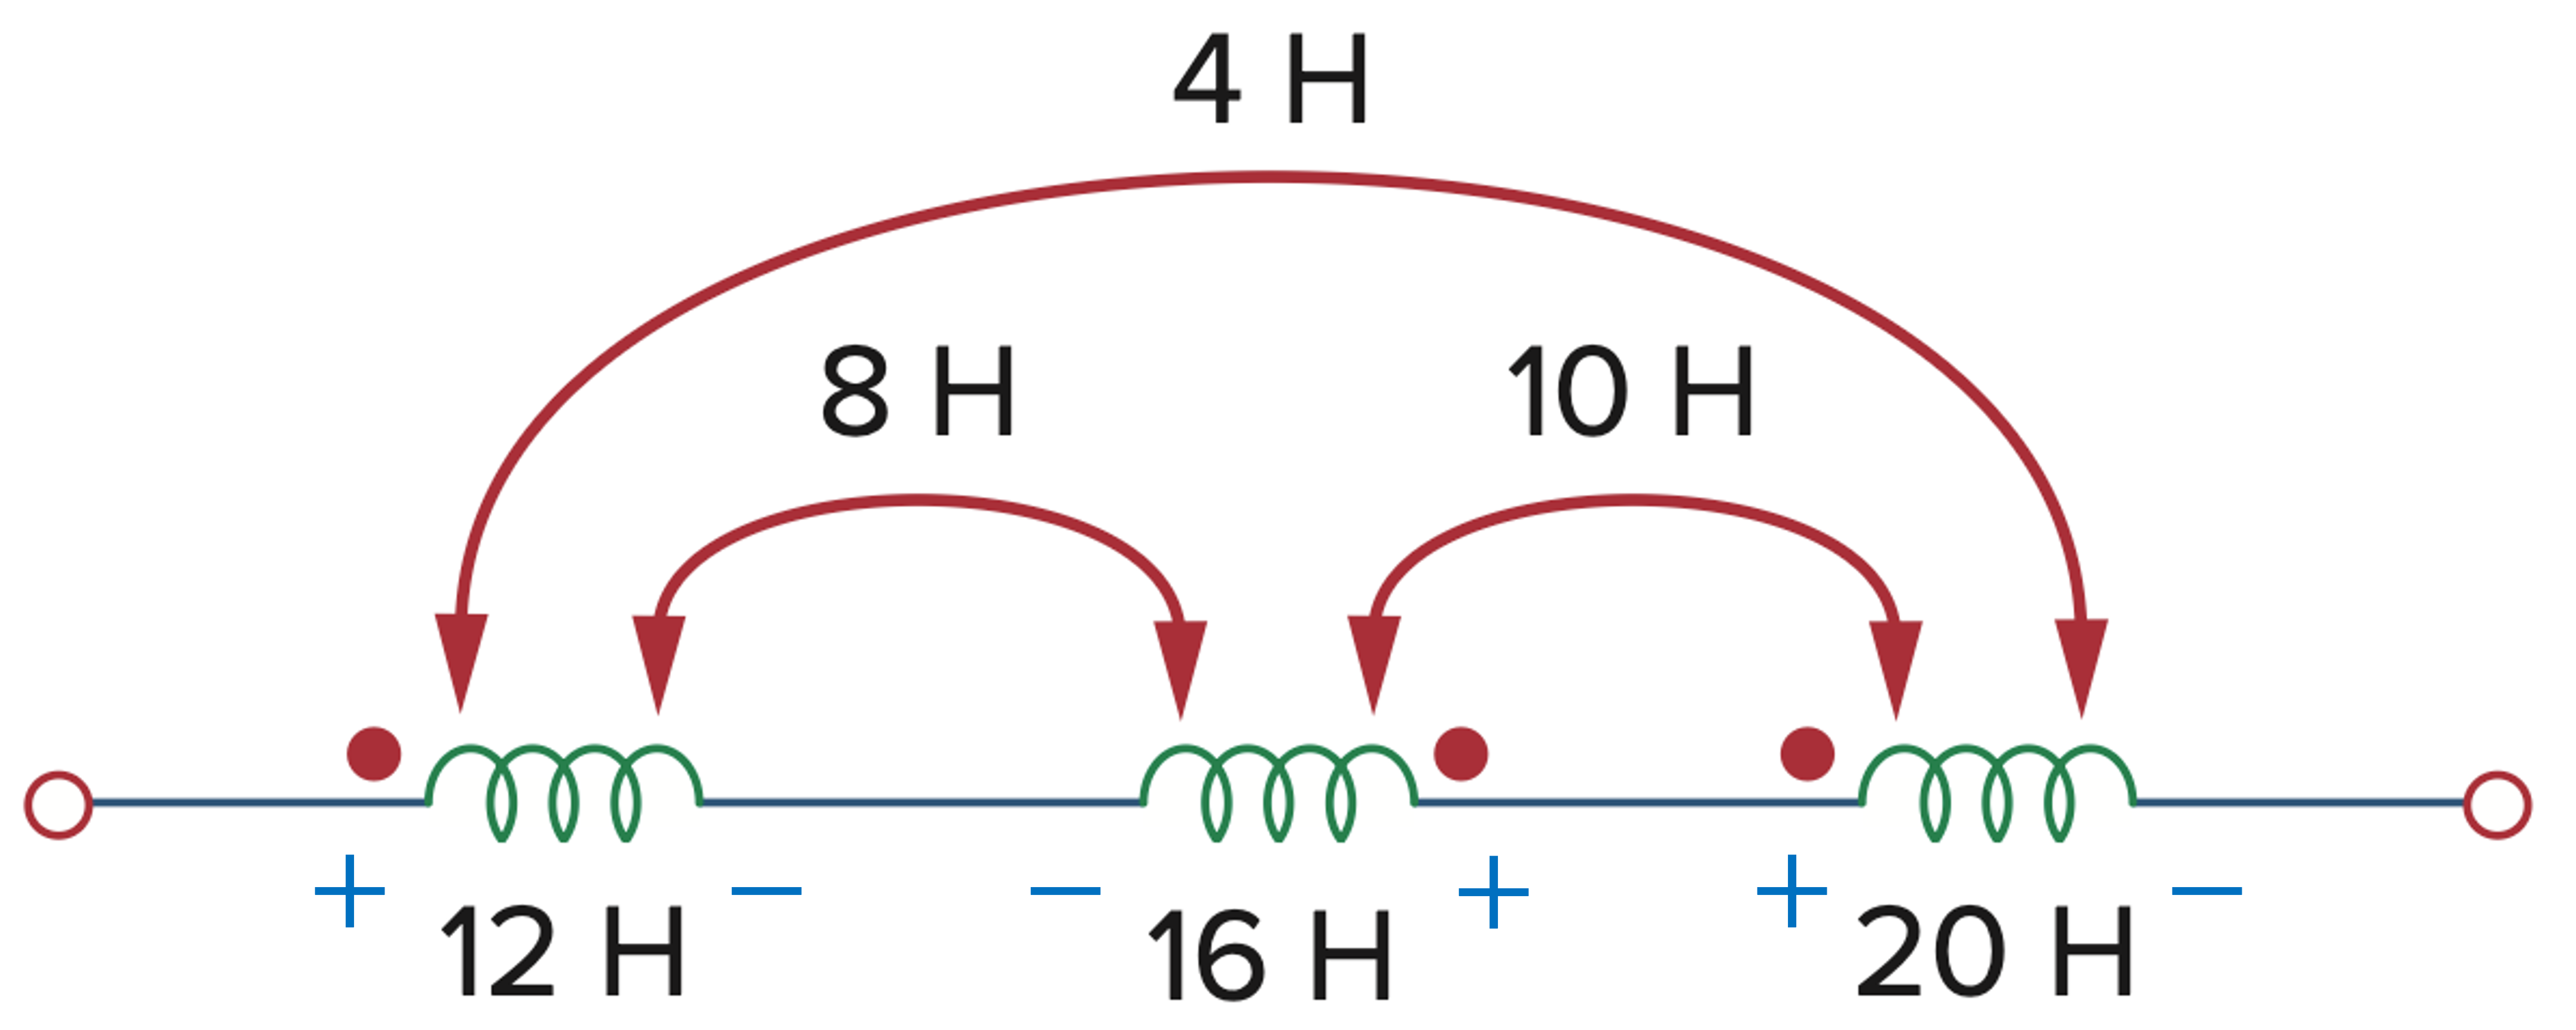
\includegraphics[width=0.7\textwidth]{figures/mutual_inductance_polarity.png}
\end{solution}
\fi

% ----- Exercise 3 -----
\begin{exercise}[RC-Entladung]
In folgender Schaltung gilt für \(t>0\)
\[
v(t) = 56e^{-200t}\,\text{V},\qquad i(t) = 8e^{-200t}\,\text{mA}.
\]
\begin{enumerate}[label=\alph*)]
  \item Bestimme \(R\) und \(C\).
  \item Berechne die Zeitkonstante \(\tau\).
  \item Bestimme die Zeit, die benötigt wird, damit die Spannung auf die Hälfte ihres Anfangswertes bei \(t=0\) abfällt.
\end{enumerate}

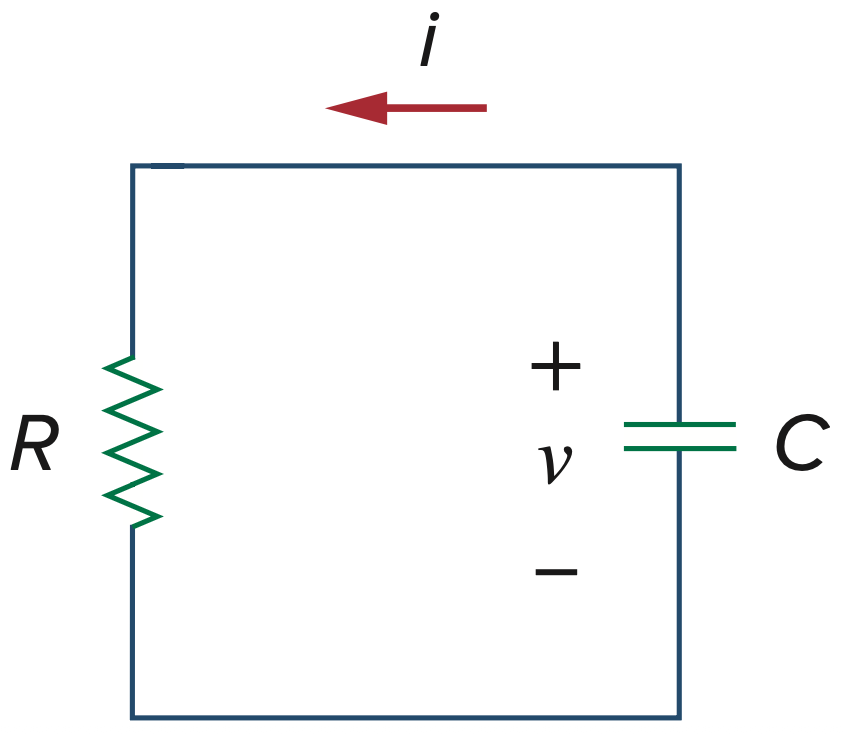
\includegraphics[width=0.5\textwidth]{figures/transients1.png}
\end{exercise}

\ifshowsolutions
\begin{solution}
\begin{enumerate}[label=\alph*)]
\item Bei einer einzelnen Reihenentladung der \(R\!-\!C\)-Schaltung hat die Kondensatorspannung die folgende Form:
\[
v(t) = V_0 e^{-t/(RC)}.
\]
Vergleich von \(v(t)=56e^{-200t}\) mit \(V_0 e^{-t/(RC)}\) ergibt
\[
\frac{1}{RC} = 200 \quad\Longrightarrow\quad RC = 5\,\text{ms}.
\]

Konsatorstrom und Kondensatorspannung hängen zusammen gemäß
\[
i(t) = C \frac{dv(t)}{dt}.
\]
Differenzieren von \(v(t)\):
\[
\frac{dv}{dt} = -200 \cdot 56 e^{-200t}\,\text{V/s} = -11200 e^{-200t}\,\text{V/s}.
\]
Somit gilt
\[
C=\frac{i(t)}{dv/dt} = \frac{0.008 e^{-200t}}{-11200 e^{-200t}}.
\]
Und da die Kapazität positiv ist,
\[
C = \frac{0.008}{11200}\,\text{F} \approx 714.3\,\text{nF}.
\]

\[
R = \frac{RC}{C} = \frac{0.005}{714.3 \times 10^{-9}}\,\Omega = 7\,\text{k}\Omega
\]
(Alternativ, \(R = v(t)/i(t) = 56/0.008\,\Omega = 7\,\text{k}\Omega\).)

\item Die Zeitkonstante ist
\[
\tau = RC = 5\,\text{ms}.
\]

\item Wir verlangen \(v(t_{1/2}) = \tfrac{1}{2}V_0\). Für \(v(t) = V_0 e^{-t/\tau}\),
\[
\frac{1}{2} = e^{-t_{1/2}/\tau}\quad\Longrightarrow\quad t_{1/2} = \tau \ln 2.
\]
Somit gilt
\[
t_{1/2} = (0.005 \cdot \ln 2)\,\text{s} \approx 3.466\,\text{ms}.
\]
\end{enumerate}
\end{solution}
\fi

% ----- Exercise 4 -----
\begin{exercise}[Zeitkonstante]
Bestimme die Zeitkonstante für folgende Schaltung.

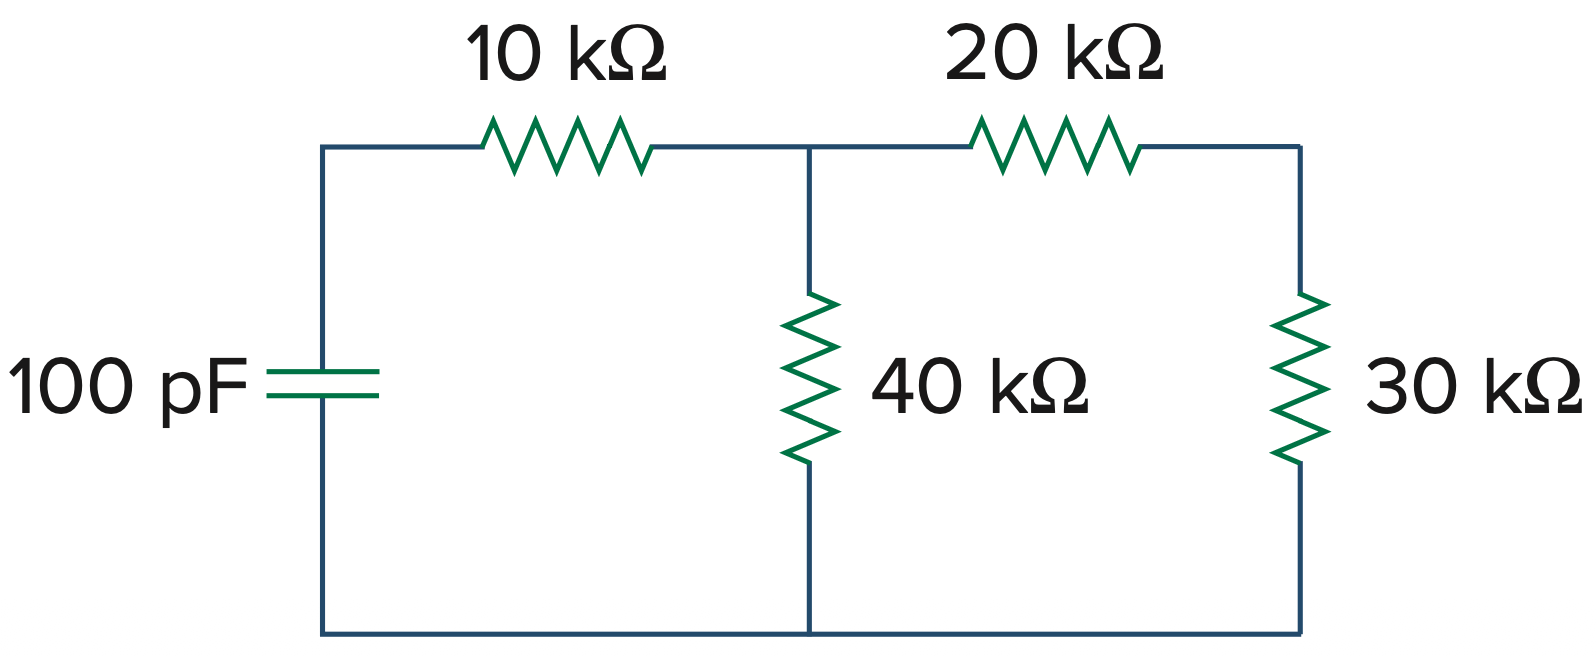
\includegraphics[width=0.7\textwidth]{figures/transients2.png}
\end{exercise}

\ifshowsolutions
\begin{solution}
Finden des Äquivalentwiderstands:
\[
R_{\text{th}} = 10~\text{k}\Omega + \left( 40~\text{k}\Omega \parallel (20~\text{k}\Omega + 30~\text{k}\Omega) \right) = 10~\text{k}\Omega + \frac{40 \cdot 50}{40 + 50}~\text{k}\Omega = \frac{290}{9}~\text{k}\Omega
\]

Berechnung der Zeitkonstanten:
\[
\tau = R_{\text{th}} C = \left( \frac{290}{9} \times 10^3~\Omega \right) \left( 100 \times 10^{-12}~\text{F} \right) = \frac{29000}{9} \times 10^{-9}~\text{s}
\]
\[
\tau \approx 3.22~\mu\text{s}
\]
\end{solution}
\fi

% ----- Exercise 5 -----
\begin{exercise}[Spulenstromabfall]
Bestimme $i_o$ für $t > 0$ in folgender Schaltung.

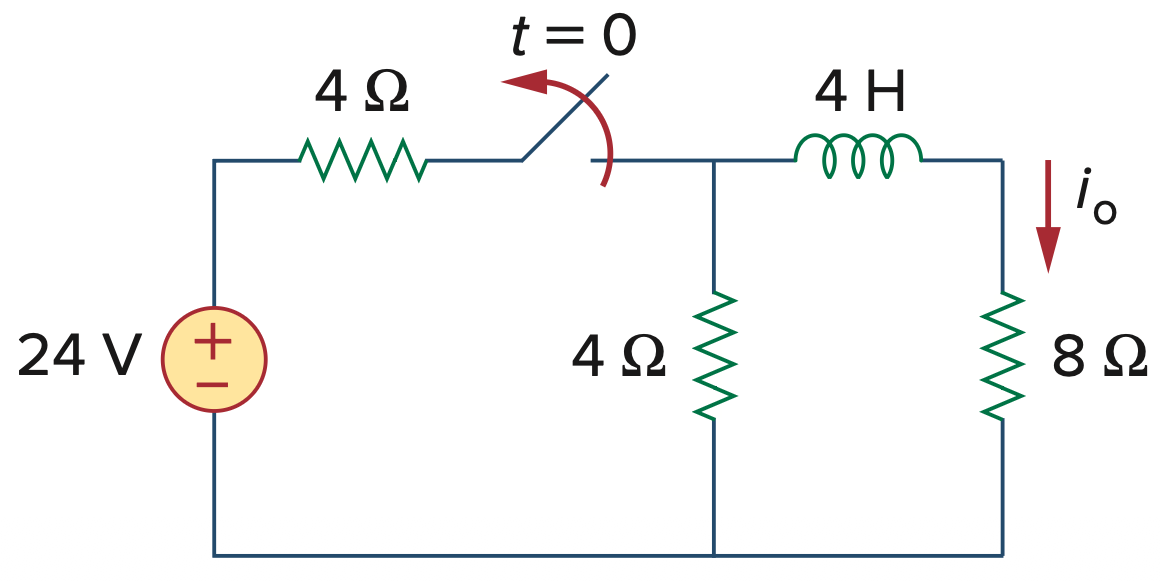
\includegraphics[width=0.7\textwidth]{figures/transients3.png}
\end{exercise}

\ifshowsolutions
\begin{solution}
Der Schalter ist für \(t<0\) geschlossen. Daher befindet sich die Induktivität im stationären Gleichstromzustand und verhält sich wie ein Kurzschluss.

Der Knoten nach dem linken \(4\Omega\)-Widerstand sieht die Parallelschaltung von \(4\Omega\) und \(8\Omega\):
\[
R_{\mathrm{eq}} = \frac{4 \cdot 8}{4+8} = \frac{8}{3}\ \Omega.
\]

Die Knotenspannung ist
\[
v(0^-) = 24\,\frac{R_{\mathrm{eq}}}{4 + R_{\mathrm{eq}}} = 24\,\frac{8/3}{4 + 8/3} = 9.6\ \text{V}.
\]

Der Spulenstrom bei \(t=0^-\) beträgt demnach
\[
i_L(0^-) = \frac{v(0^-)}{8} = \frac{9.6}{8} = 1.2\ \text{A}.
\]

Somit ist
\[
i_L(0^+) = 1.2\ \text{A}.
\]

Nach dem Öffnen des Schalters bei \(t=0\) wird die Stromquelle getrennt. Der obere Knoten ist dann nur mit einem \(4\Omega\)-Widerstand gegen Masse und der Induktivität mit \(L=4\,\mathrm{H}\) in Reihe mit einem \(8\Omega\)-Widerstand verbunden.

Anwendung der Kirchhoffschen Knotenregel am oberen Knoten (Ströme fließen nach unten positiv):
\[
\frac{v}{4} + i_L = 0
\]

Somit gilt
\[
v = -4 i_L.
\]

Die Spannung des rechten Zweigs ist auch
\[
v = 8 i_L + L \frac{di_L}{dt} = 8 i_L + 4\frac{di_L}{dt}.
\]

Gleichsetzen der beiden Ausdrücke für \(v\):
\[
-4 i_L = 8 i_L + 4\frac{di_L}{dt}
\]

Teilen durch 4:
\[
\frac{di_L}{dt} + 3\, i_L = 0.
\]

Somit ist
\[
i_L(t)= i_L(0^+)\, e^{-3t} = 1.2\, e^{-3t}.
\]

\[
\boxed{i_o(t)=1.2\,e^{-3t}\ \text{A},\quad t>0.}
\]
\end{solution}
\fi

% ----- Exercise 6 -----
\begin{exercise}[Energiedissipation beim Entladen]
In foldender Schaltung gilt
\[
v(t)=80e^{-10^{3}t}\ \text{V},\qquad t > 0,
\]
\[
i(t)=5e^{-10^{3}t}\ \text{mA},\qquad t > 0.
\]

\begin{enumerate}[label=\alph*)]
  \item Bestimme \(R,\ L,\ \tau\).
  \item Berechne die im Widerstand umgesetzte Energie für \(0 < t < 0.5\,\text{ms}\).
\end{enumerate}

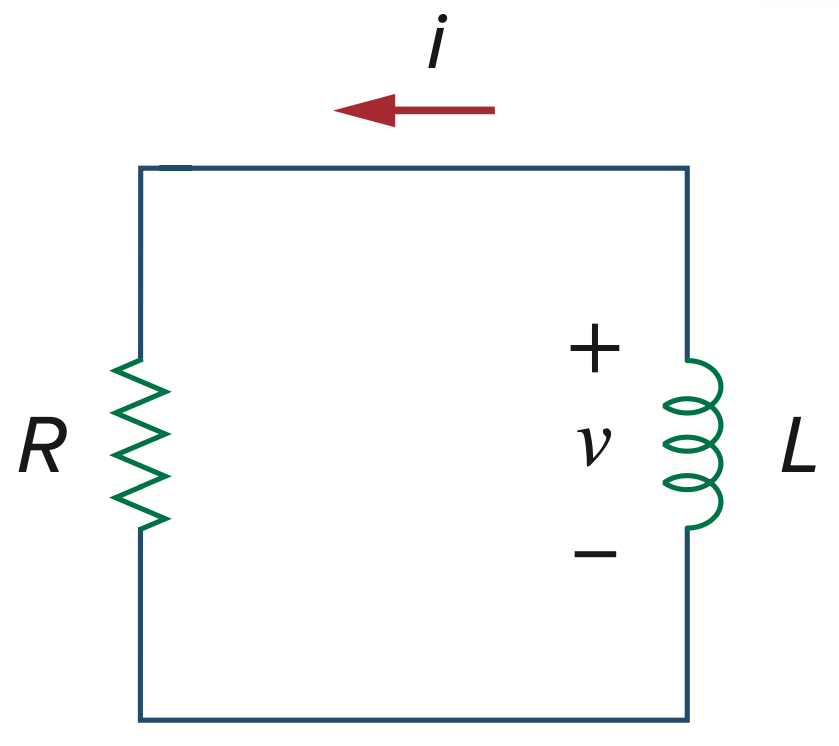
\includegraphics[width=0.7\textwidth]{figures/transients4.png}
\end{exercise}

\ifshowsolutions
\begin{solution}
\begin{enumerate}[label=\alph*)]
\item Der Strom hat die Form \(i(t)=I_0 e^{-t/\tau}\). Der Vergleich der Exponenten ergibt
\[
\frac{1}{\tau}=1000\quad\Longrightarrow\quad \tau = 1\,\text{ms}.
\]

Da die Spannung \(v(t)\) auch am Widerstand anliegt, gilt
\[
R = \frac{v(t)}{i(t)} = \frac{80e^{-1000t}}{5\times10^{-3}e^{-1000t}} = 16\,\text{k}\Omega.
\]

Demnach ist
\[
L=\tau R=(1\times10^{-3})(1.6\times10^{4}) = 16\,\text{H}.
\]

\item Die in \(R\) umgesetzte Energie von \(t=0\) bis \(t=t_1\) beträgt
\[
W=\int_{0}^{t_1} i^2(t)\,R\,dt, \qquad t_1 = 0.5\,\text{ms}.
\]
Somit gilt
\[
W=R\int_0^{t_1} (5\times10^{-3})^2 e^{-2000t}\,dt = R\,(25\times10^{-6})\int_0^{t_1} e^{-2000t}\,dt.
\]
Auswerten des Integrals:
\[
\int_0^{t_1} e^{-2000t}\,dt=\left[-\frac{1}{2000}e^{-2000t}\right]_0^{t_1} =\frac{1}{2000}\big(1-e^{-2000t_1}\big).
\]
Somit ist
\[
W=R\,(25\times10^{-6})\frac{1}{2000}\big(1-e^{-2000t_1}\big).
\]
Einsetzen von \(R=1.6\times10^{4}\) und \(2000t_1=2000(5\times10^{-4})=1\):
\[
W=(1.6\times10^{4})(25\times10^{-6})\frac{1}{2000}\big(1-e^{-1}\big) = 1.26424\times10^{-4}\,\text{J} \approx 0.126\ \text{mJ}.
\]
\end{enumerate}
\end{solution}
\fi

\end{document}